\section{Tomassini Antonioni Models}

\subsubsection{Introduction}
This chapter will discuss the analysis of PGGs on networks using the model developed by Marco Tomassini and Alberto Antonioni in \cite{RN49}. First, their model is replicated, and the replicated results are compared to the published results. Then the replicated results are examined for robustness. After that, the analysis is extended to further graph types to analyse the effect of graph structure on cooperation. \\

\subsection{Payoff Satisfaction Model}
This model is described in \cite{RN49} and emulates an agent who increases their contribution when they are \emph{satisfied}. The goal is to accurately reflect results observed in human experiments. This differs strongly from evolutionary dynamics, which will be discussed in a later chapter. The payoff $\pi_i$ of an individual $i$ enrolled in $g_i$ groups each with size $|N_j|$ is \\
\begin{align} 
    \pi_i(c_i) = g_i(1-c_i) - g_ic_i + \sum_{j=1}^{g_i} \sum_{k=1}^{|N_j|} \frac{rc_k}{|N_j|}, \quad c_i \in C:= \{0.0, 0.25, 0.50, 0.75, 1.0\}. 
\end{align}

It is enforced that each player contributes a constant $c_i$ to each group, and is initially endowed with $g_i$ units. The first term is their endowment after contribution, the second term is their contribution and the last term represents the enhanced return earned from all the games. \\

Each agent's initial contribution is randomly chosen from the set $C$. The choice set qualitatively emulates a lab experiment, where players are given tokens and choose how many to contribute. \\

The agents' update rule is simple. If they receive, from the common pools, at least as much as they contribute, they are \emph{satisfied}, and increase their contribution by 0.25 with probability 0.5, otherwise remain unchanged. In the case where they are \emph{unsatisfied}, their contribution always decreases by 0.25. Obviously an agent playing $c_i =1$ cannot increase their contribution, and similarly an agent playing $c_0$ cannot decrease their contribution. This model does not claim to simulate evolutionary dynamics, instead to replicate results observed in human trials. \\


\subsection{Network Structure}
Antonioni and Tomassini developed their own model for the generation of social networks in the paper \cite{RN51}. This model considers the degree of vertices as well as their location in two--dimensional unitary space $[0,1]^2$. Similar to the Barab\'{a}si--Albert model described in \ref{BA}, a growing mechanism is used to create the graph. The parameters are $N$, the population size, $k$, the targeted mean degree, and $\alpha$, a mixing parameter. \\

The graph is initialised with a clique of $k+1$ nodes distributed in $[0.45, 0.55]^2$. Then each new node is added randomly in $[0,1]^2$ and prescribed a number of links drawn from $\mathsf{DU}(1,2k-1)$. For each link, a uniform random number is compared to the parameter $\alpha$. If the random number is less than $\alpha$, the node is then joined to an existing node chosen by preferential attachment as in a Barab\'{a}si--Albert model. Otherwise, the node is joined to the geometrically closest existing node that is not already linked. \\

The paper \cite{RN51} compares graphs built using this model to real--world graphs, and finds it exhibits the common features for a social network. Relative to a Barab\'{a}si--Albert model, the clustering coefficient is higher due to the spatial dimension. It also preserves the right-skewed degree distribution and low path lengths. \\

This network model serves as the structure for the game in \cite{RN49}, with agents stationed at nodes.

\subsection{Results Comparison}
The results obtained were compared to the results reported in the paper \cite{RN49}. The comparison is shown in Figure \ref{comp0}. Evidently, increasing the enhancement factor $r$ increases cooperation. It is interesting to note that equilibrium is reached relatively quickly ($\sim$ 20 rounds). In \cite{RN49}, the authors note that even in the case of low $r$, zero cooperation is not observed. This agrees with experimentally reported results, but disagrees with classical and evolutionary game theory predictions. In fact, the minimum contribution amount 0.0835 can be shown analytically as a steady state. For simplification, assume the agent is playing $g=7$ games, each with $|N_j|=7$, $j=1, \dots, 7$ agents in a game. If the population is contributing 0.0835 on average, then  an agent contributing 0 will have expected return $$ \mathbb E \sum_{j=1}^{g_i} \sum_{k=1}^{|N_j|} \frac{rc_k}{|N_j|} =   7*\frac{1.8*0.0835*6 + 0*1}{7} =  0.90 >7*0,$$ so they will be \emph{satisfied}, and increase their contribution to 0.25 with probability 0.5. If they are contributing 0.25, their expected return is 
$$ \mathbb E \sum_{j=1}^{g_i} \sum_{k=1}^{|N_j|} \frac{rc_k}{|N_j|} =7* \frac{1.8*0.0835*6 + 0.25}{7} = 1.152< 0.25*g  =1.75, $$
 and hence they will be\emph{unsatisfied}, and reduce their contribution to 0. This is a Markov process for states 0, 0.25. The transition matrix $\mathbf{P}$, is $$\mathbf P = \begin{bmatrix} 0.5& 0.5 \\
1& 0 \\
\end{bmatrix}. $$ The stationary distribution solves $\pi \mathbf{P} = \pi$. For $\mathbf{P}$ defined above, $\pi = [\tfrac{2}{3}, \tfrac{1}{3}]$, which corresponds to a mean degree of 0.0833, well within computational error. 

\FloatBarrier 
\begin{figure}[!h]
  \begin{subfigure}[b]{0.45\textwidth}
    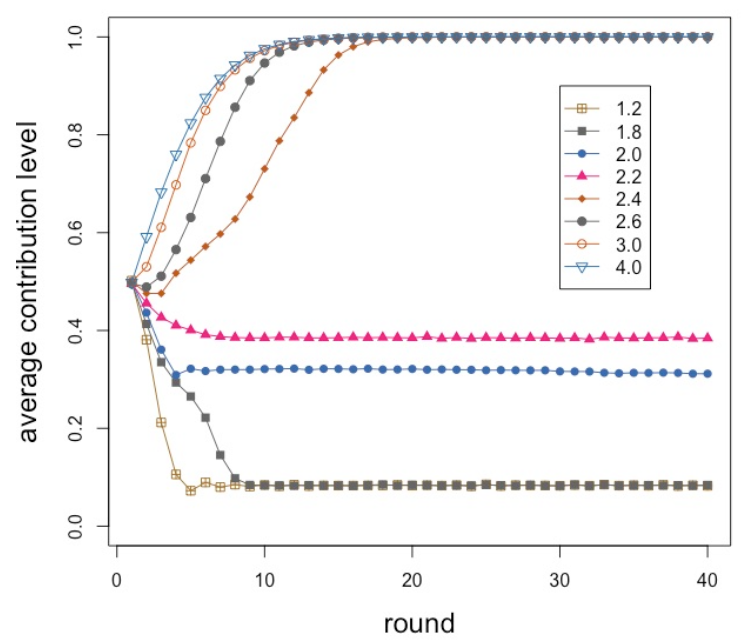
\includegraphics[width=\textwidth]{images/TAfig2_real.png}
    \caption{Figure 2 from \cite{RN49}. }
    \label{TAfig2_real}
  \end{subfigure}
  \hfill
  \begin{subfigure}[b]{0.45\textwidth}
    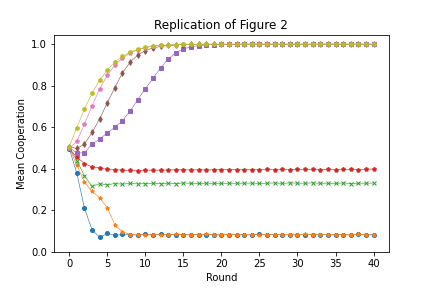
\includegraphics[width=1.25\textwidth]{images/TAfig2.png}
    \caption{Replication of \ref{TAfig2_real}. }
    \label{TAfig2}
  \end{subfigure}
  \caption{Comparison of reported results from \cite{RN49} and replicated results. Each series represents a value for the enhancement factor $r \in [1.2, 1.8, 2.0, 2.2, 2.4, 2.6, 3.0, 4.0]$, which corresponds to blue circles, orange stars, green crosses, red pentagons, purple squares, brown diamonds, pink pentagons, and olive hexagons respectively. They appear almost identical, indicating that the replication is successful.} \label{comp0}
\end{figure} 
\FloatBarrier

For further confirmation, Figures 5a and b from the paper were also replicated, shown in Figures \ref{comp1}, and \ref{comp2}. These correspond to modifying the underlying graph to a purely spatial ($\alpha = 0$), or preferential attachment ($\alpha = 1)$ model. The similarity of these results indicates both the agent and graph models correctly replicate the descriptions given in \cite{RN49}.

\FloatBarrier
\begin{figure}[!h] 
  \begin{subfigure}[b]{0.45\textwidth}
    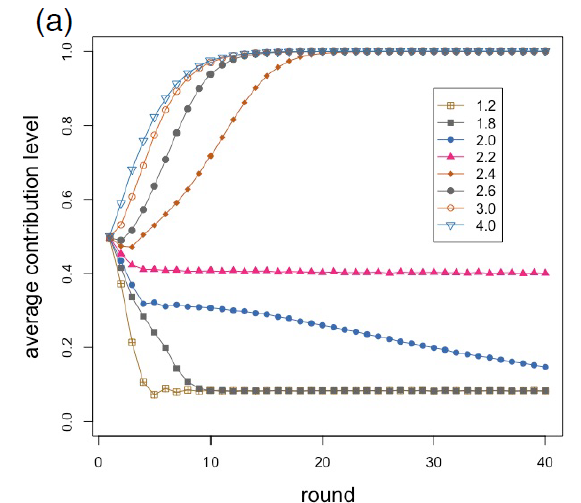
\includegraphics[width=\textwidth]{images/TAfig4a_real.png}
    \caption{Figure 5a from \cite{RN49}. $\alpha = 0$ }
    \label{TAfig4a_real}
  \end{subfigure}
  \hfill
  \begin{subfigure}[b]{0.45\textwidth}
    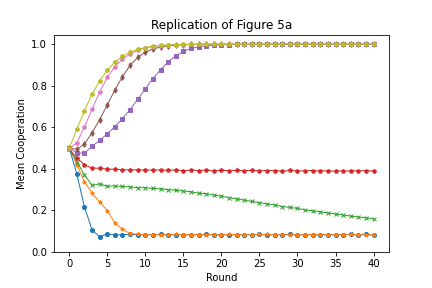
\includegraphics[width=1.35\textwidth]{images/TAfig4a.png}
    \caption{Replication of \ref{TAfig4a_real}. }
    \label{TAfig4a}
  \end{subfigure}
  \caption{Comparison of reported results from \cite{RN49} and replicated results. Each series represents a value for the enhancement factor $r \in [1.2, 1.8, 2.0, 2.2, 2.4, 2.6, 3.0, 4.0]$, which corresponds to blue circles, orange stars, green crosses, red pentagons, purple squares, brown diamonds, pink pentagons, and olive hexagons respectively. Once again, the replication is successful. } \label{comp1}
\end{figure} 
\FloatBarrier




\FloatBarrier
\begin{figure}[!h] 
  \begin{subfigure}[b]{0.45\textwidth}
    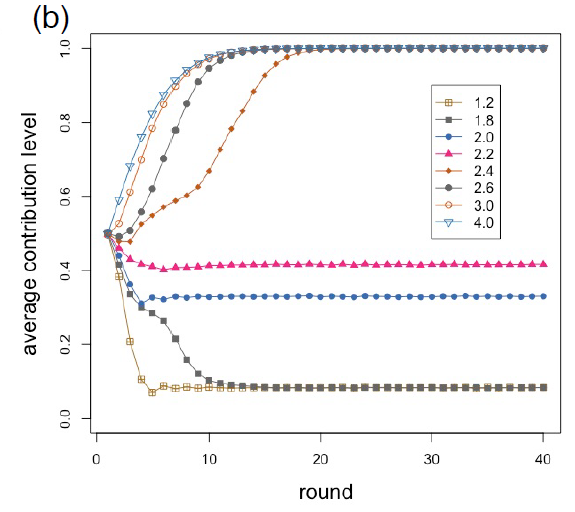
\includegraphics[width=\textwidth]{images/TAfig4b_real.png}
    \caption{Figure 5b from \cite{RN49}. $\alpha = 1$ }
    \label{TAfig4b_real}
  \end{subfigure}
  \hfill
  \begin{subfigure}[b]{0.45\textwidth}
    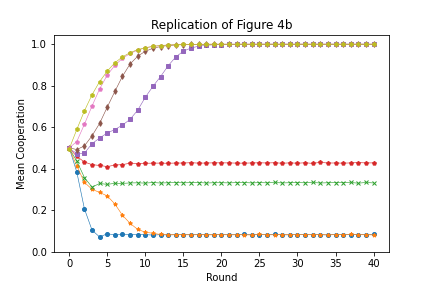
\includegraphics[width=1.35\textwidth]{images/TAfig4b.png}
    \caption{Replication of \ref{TAfig4b_real}. }
    \label{TAfig4b}
  \end{subfigure}
  \caption{Comparison of reported results from \cite{RN49} for $\alpha = 1$. Each series represents a value for the enhancement factor $r \in [1.2, 1.8, 2.0, 2.2, 2.4, 2.6, 3.0, 4.0]$, which corresponds to blue circles, orange stars, green crosses, red pentagons, purple squares, brown diamonds, pink pentagons, and olive hexagons respectively. } \label{comp2}
\end{figure} 
\FloatBarrier

They key results from \cite{RN49} have been reproduced. Other results from their paper, where the mean degree is varied, have also been reproduced, but are not included for the sake of brevity.\\


\subsection{Robustness}
The robustness of results was discussed qualititatively in \cite{RN49}, and the authors demonstrated consistency in results. However no quantitative analysis was provided. To examine the variance in the results, the number of trials, $T$ was increased to 120. The first plot examines the shape of the distribution for each of the series by plotting the empirical 2.5\% and 97.5\% quantiles. \\

\FloatBarrier
\graphCap{sensitivity2.png}{0.8}{2.5\% and 97.5\% quantiles for each series. Each series represents a value for the enhancement factor $r \in [1.2, 1.8, 2.0, 2.2, 2.4, 2.6, 3.0, 4.0]$, which corresponds to blue, orange, green, red, purple, brown, pink, and olive respectively. The mean is shown as a solid line, and the quartiles as dashed. Only 6 out of 120 trials lie outside the dashed lines for each series.}{sens2}
\FloatBarrier
The series corresponding to $r=2.2$ shows a 97.5\% quantile trend of around 0.58. This is much higher than the mean trend. This shows the influence of the particular network within the network model, particularly for the critical values at which cooperation is sustained but full cooperation is not achieved. It is interesting to note that this phenomenon does not occur for the $r=2$ line, which also achieves incomplete but non-zero cooperation. For $r \in [2.2, 2.28]$, the 2.5\% quantile is the same, however the mean trends are different. There appears to be a lower bound of 0.33, which represents a population switching between 0.25 and 0.5 similar to the lower bound of 0.0835 discussed in reference to \ref{comp0}. The image below applies the Central Limit Theorem to the cooperation level, and plots a $95\%$ confidence interval for the mean for each series. The Central Limit Theorem derives a 95\% CI for the mean, as $\pm 1.96*\frac{\sigma}{\sqrt{T}}$, where $\sigma$ is the empirical standard deviation. The Central Limit Theorem is applicable, as there are more than 30 samples for each series. \\
\FloatBarrier
\graphCap{sensitivity1.png}{0.8}{95\% Confidence interval for the mean of each series. Each series represents a value for the enhancement factor $r \in [1.2, 1.8, 2.0, 2.2, 2.4, 2.6, 3.0, 4.0]$, which corresponds to blue, orange, green, red, purple, brown, pink, and olive respectively. The mean is shown in the solid line, and the bounds of the confidence interval are shown as dashed lines. It is evident that the results are stable. Only the middle series, $r=2.2$, shows some variance.}{sens1}
\FloatBarrier
The image shows that the means are stable, and the results are robust. The confidence intervals for the mean are symmetric about the mean, due to the assumption of limiting normality. \\

To investigate the effect of network structure on cooperation, the Tomassini Antonioni model will be extended to other network models. \\

\subsection{Extension to Other Network Models}

In \ref{RG}, three main network models are discussed. These are the Erd\H{o}s--R\'enyi graph, \emph{small-world} network (WS), and also the Barab\'{a}si--Albert (BA) model. In the following analysis, $G(n,r)$ graphs are chosen for Erd\H{o}s--R\'enyi graphs, and denoted RRG (random regular graphs). This is to be able to control the mean degree. All three of these network models are implemented using the \verb+networkx+ Python package. For comparison, the model described by Tomassini and Antonioni in \cite{RN51} is included, and denoted Tomassini Antonioni Graph (TAG). \\

Small--world networks actually describe a family of graphs, depending on the parameter $p$. For this analysis, $p$ was set to 0.1, which preserves local clustering and reduces the average shortest path length. Importantly, only connected WS graphs are used. If the graph generated is not connected, then a new one with the same parameter is generated until they are connected. This is convention to allow strategies to propagate throughout the graph. \\

Similarly, TAG is a family of graphs. In the plots below, the proportion parameter $\alpha$ is set to 0.3, as recommended by \cite{RN49}. Firstly, a sample of 100 graphs for each model were taken, and their descriptive statistics were computed. \\


\FloatBarrier

    

\begin{table}[!h]
\begin{center}
\begin{tabular}{|l|l|l|l|l|}
\hline
Graph Type & Mean Degree & $l$ & $C_\Delta$ & Degree Variance \\ \hline
BA         & 5.96        & 3.24                         & 0.05                   & 40.80           \\ \hline
RRG        & 6           & 3.75                         & 0.01                   & 0               \\ \hline
TAG        & 5.99        & 3.84                         & 0.22                   & 16.95           \\ \hline
WS         & 6           & 5.39                         & 0.44                   & 0.57            \\ \hline
\end{tabular}
\caption{Computed characteristics for BA, RRG, TAG, and WS models. The characteristics were computed over 100 samples of each graph, and then averaged. } \label{graph_stats}
\end{center}
\end{table}

\FloatBarrier

The degree variance does not accurately describe all the facets of the degree distribution, so a histogram for each model is plotted below. For each graph model, 10 graphs were created according to the previously described parameters and their degree counts summed to create the histograms. \\
\FloatBarrier
\graphCap{hist1.png}{0.7}{Degree Histogram for WS and RRG models. The RRG model enforces a degree of 6 for every node. The WS model starts from a lattice, then rewires each link with probability $p$.}{hist1}
\FloatBarrier
\graphCap{hist2.png}{0.7}{Degree Histogram for BA and TAG models, on a logarithmic scale. The logarithmic scale clearly shows the counts for higher degrees. Because the TAG model uses preferential attachment only $\alpha = 0.3$ proportion of the time, it is not a true scale--free distribution. }{hist2}
\FloatBarrier
One of the goals of the TAG was to preserve a higher clustering coefficient than BA graphs, while remaining approximately scale--free. Table \ref{graph_stats} emphasises this effect. From these descriptive statistics, it appears that BA and RRG can be considered similar except for their degree distributions. The mean cooperation level for each graph was plotted. Because this is novel analysis, the number of trials $T$ was set to 80, and each trial observes 60 steps. \\

\FloatBarrier
\graphCap{graphs1.png}{0.8}{Comparing Models, $1.85 \leq r \leq 2.0$. In each graph, the blue, orange, green, red lines correspond to the WS model, TAG model, BA model, and RRG model respectively. For $r<1.85$, minimal cooperation is observed, so these plots are not shown. It is observed that first RRG, then BA, then TAG, then WS achieve non--trivial cooperation. This corresponds to the order of increasing $C_\Delta$. }{graphs11}
\FloatBarrier

It appears that $C_\Delta$ dictates the value for $r$ for which non--trivial cooperation is observed. Interestingly, for $\alpha = 0.3$, 30\% of the TAG graph are nodes added in BA style. Yet the TAG graph follows the trend of the WS model more than the BA model.
\FloatBarrier
\graphCap{graphs2.png}{0.8}{Comparing Graph models, $2.25\leq r \leq 2.4$. In each graph, the blue, orange, green, red lines correspond to the WS model, TAG model, BA model, and RRG model respectively. For $2.0<r<2.25$, the cooperation levels were very similar around 0.5.  It is an almost perfect trend reversal, as WS is the first graph to achieve full cooperation, then TAG, then BA and finally RRG. For $r>2.4$, full cooperation was always achieved. \\ }{graphs1}
\FloatBarrier
For higher ranges of $r$, it is more interesting. The WS and TAG trends achieve full cooperation earlier. This seems to indicate that the agents are more uniform under this graph structure. The WS and TAG models have a small range of $r$ for which non--trivial cooperation is observed. These graph models also have high $C_\Delta$, which may propagate strategies through the population, and enforce homogeneity in contribution. Both the WS and RRG model have very low degree variance, yet behave quite differently. It appears that the degree distribution does not impact the cooperation level for Tomassini Antonioni style agents. \\

\subsection{Summary}

This chapter focussed exclusively on agents defined by Tomassini and Antonioni in \cite{RN49}. Tomassini and Antonioni demonstrated that these agents are a good proxy for human interactions, and simulated the Public Goods Game on a custom network model. These results were perfectly replicated, and both plots are shown in Figures \ref{comp0}, \ref{comp1}, \ref{comp2}.  A lower bound of 0.0835 was demonstrated analytically. The robustness of these results were also examined. It is shown that 120 repetitions were sufficient to estimate the mean of each series, however the empirical quantile plots showed that there is quite high variance in distribution for the series corresponding to $r=2.2$.\\ 

The agents from this model were then tested on different models for random graphs. The results are interesting in the range $1.85\leq r \leq 2.4$. The trend indicates that models with high clustering coefficient $C_\Delta$ do not support intermediate levels of cooperation, and remain at the lower bound of cooperation for higher $r$ and full cooperation for lower $r$ relative to models with low $C_\Delta$. Other characteristics of the graph model, such as degree distribution and ASPL did not seem to have an effect. \\



